\documentclass[serif,xcolor=pdftex,dvipsnames,table,hyperref={bookmarks=false,breaklinks}]{beamer}

%%%%%%%%%%%%%%%%
% Change the macros below to configure the title slides
% for your course.
\newcommand{\coursename}{COMPSCI 589}
\newcommand{\instructor}{Benjamin M. Marlin}
\newcommand{\university}{University of Massachusetts Amherst}
\newcommand{\department}{College of Information and Computer Sciences}
%%%%%%%%%%%%%%%%


\newcommand{\settitlecard}[2]{
  \title[\coursename  Lecture #1] 
    {\coursename \\ Lecture #1: #2}
     \author[\instructor]{\instructor}
     \institute[\university]{
     \department\\
     \university
   }
\date{}
}

\newcommand{\maketitlepage}{
  \begin{frame}
  \titlepage
  \center{
    %If you use the slides unmodified, retain the attribution below
    \tiny{Slides by Benjamin M. Marlin (marlin@cs.umass.edu). \\
    \vspace{-1em}Created with support from National Science Foundation Award\# IIS-1350522. 
    %If you modify the slides, please retain the alternate attribution below
    %\tiny{Based on slides by Benjamin M. Marlin (marlin@cs.umass.edu). \\    
    %\vspace{-1em}Created with support from National Science Foundation Award\# IIS-1350522. 
    }                                              
  }  
  \end{frame}
}

\AtBeginSection[]
{
  \begin{frame}<beamer>{Outline}
    \tableofcontents[currentsection,subsectionstyle=hide]
  \end{frame}
}


\newcommand{\cut}[1]{}

\newcommand{\iconbox}[4]{
  \only<#1-#2>{
    \begin{columns}[T]
      \column{0.5in}
           \includegraphics[width=0.5in]{#3}
       \column{3.7in}
            #4
    \end{columns}
    \medskip
    \medskip
    \medskip
  }
}

\mode<presentation>{
  \usepackage{../beamertheme589theme}
  \setbeamercovered{invisible}
}

\mode<handout>{
  \usepackage{../beamertheme589theme}
  \setbeamercovered{transparent}
}


\usepackage[english]{babel}
\usepackage[latin1]{inputenc}
\usepackage{times}
\usepackage[T1]{fontenc}
\usepackage{amsmath}
\usepackage{amssymb}
\usepackage[noend]{algorithmic}
\usepackage{algorithm}
\usepackage{listings}

\renewcommand\mathfamilydefault{\rmdefault}

\newcommand{\setA}{\mathcal{A}}
\newcommand{\setB}{\mathcal{B}}
\newcommand{\setS}{\mathcal{S}}
\newcommand{\setV}{\mathcal{V}}
\DeclareMathOperator*{\union}{\bigcup}
\DeclareMathOperator*{\intersection}{\bigcap}
\DeclareMathOperator*{\Val}{Val}
\newcommand{\mbf}[1]{{\mathbf{#1}}}
\DeclareMathOperator*{\argmax}{arg\,max}
\DeclareMathOperator*{\argmin}{arg\,min}
\DeclareMathOperator*{\sign}{sign}
\newcommand{\deriv}[2]{\frac{\partial{#1}}{\partial{#2}}}


\settitlecard{10}{Support Vector and Neural Network Regression}

\begin{document}

\maketitlepage

\section{SVR}
\subsection{foo}

\begin{frame}[t]{Support Vector Regression}

\begin{itemize}
\item Support Vector Regression (SVR) is the generalization of SVMs to the case of regression.

\pause \item As with SVMs, SVR is a linear regression model trained using a different objective function. In this case, the \textit{epsilon insensitive loss}.
\end{itemize}
\pause
\center
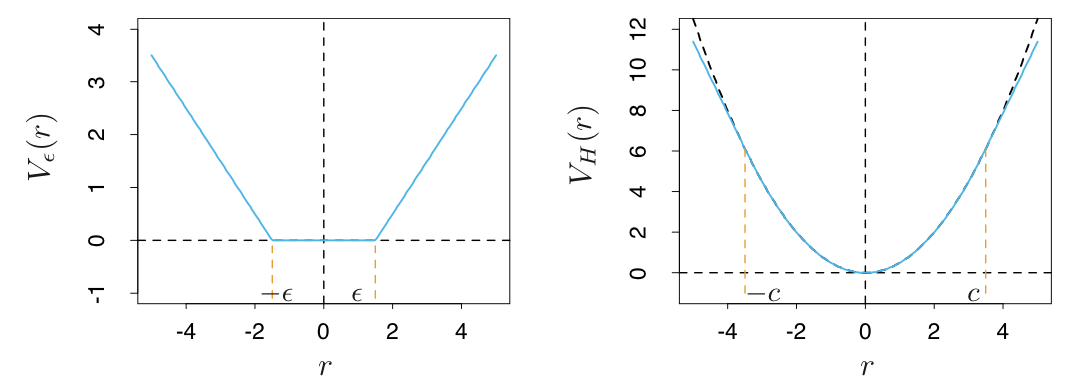
\includegraphics[width=4in]{../Figures/svr_loss.png}

\end{frame}

\begin{frame}[t]{Support Vector Regression}

$$f_{SVR}(\mbf{x}) = \left(\sum_{d=1}^D w_d x_d\right) + b = \mbf{x}\mbf{w}+b$$

\pause
$$\mbf{w}^*,b^* = \argmin_{\mbf{w},b} C\sum_{i=1}^N V_{\epsilon}(y_i - \mbf{x}_i\mbf{w}-b) + ||\mbf{w}||_2^2$$

\pause
$$V_{\epsilon}(r) = 
\left\{
\begin{array}{lr}
0 & \mbox{ ... if } |r|<\epsilon\\
|r|-\epsilon & \mbox{ ... otherwise }
\end{array}
\right.
$$
\end{frame}

\begin{frame}[t]{Support Vector Regression}

\center
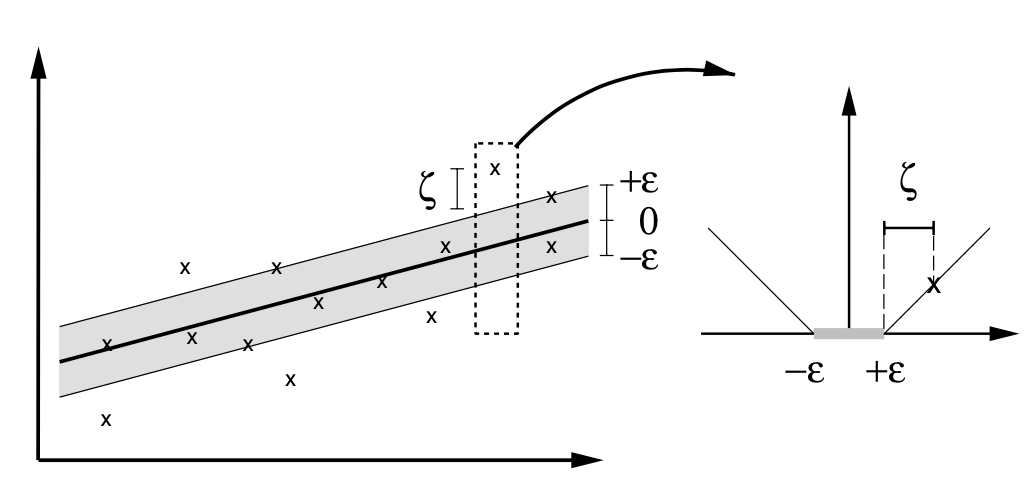
\includegraphics[width=4in]{../Figures/svr_example.png}

\end{frame}

\begin{frame}[t]{Kernelization}

Using the same representer theorem used in classification, it can be shown that

$$f_{SVR}(\mbf{x}) = \mbf{x}\mbf{w}^*+b* = \sum_{i=1}^N \alpha_i<\mbf{x},\mbf{x}_i> + \sum_{i=1}^N \alpha_i<1,\mbf{x}_i>$$

\pause This can again be generalized using kernels to allow for non-linear models:
$$f_{SVR}(\mbf{x}) = \mbf{x}\mbf{w}^*+b* = \sum_{i=1}^N \alpha_iK(\mbf{x},\mbf{x}_i)$$


\end{frame}

\begin{frame}[t]{SVR vs KRR}
\center
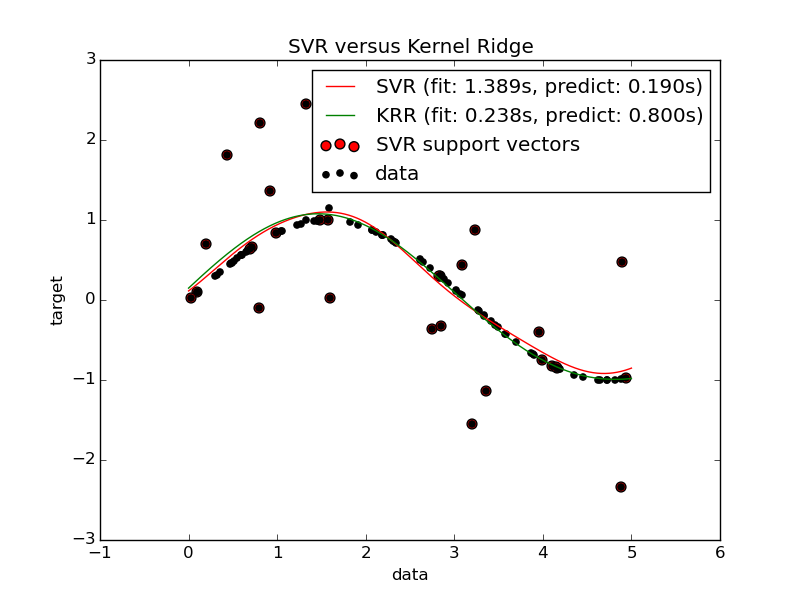
\includegraphics[width=3.5in]{../Figures/svr_vs_krr.png}
\end{frame}

\begin{frame}[t]{Trade-Offs}

\begin{itemize}
\item SVR is more robust to outliers than OLS (minimizing the MSE) due to the loss being linear in the tails instead of quadratic. This is related to a long line of work on robust regression.

\pause \item Kernel SVR is low bias and has good capacity control, but use of
cross validation to select regularization hyperparameters is critical.

\pause\item The learning problem is convex for any choice of 
reglarization parameters and thus has a unique global optimum.

\pause\item The kernel matrix computation is quadratic in the data dimension,
but the model has a support vector property.

\pause\item You need to know what kernel to use or you need to
use some form of validation to select from among several alternatives.

\end{itemize}

\end{frame}


\section{Neural Network Regression}
\subsection{foo}

\begin{frame}[t]{Multi-Layer Perceptron}

\center
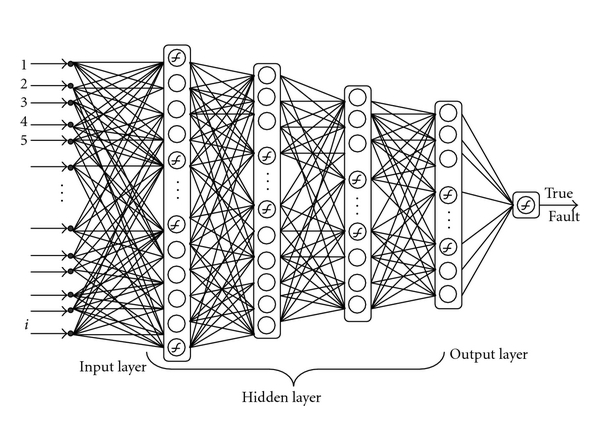
\includegraphics[width=4in]{../Figures/sigmoid_network.jpg}

\end{frame}


\begin{frame}[t]{Neural Network Regression}
To convert an MLP from classification to regression, we only need to change the output
activation function from logistic to linear.
\begin{itemize}
\setlength{\itemsep}{12pt}

\item The hidden layer non-linearities are smooth functions:

\begin{align*}
h^{1}_k &= \frac{1}{1+\exp(-(\sum_{d}w_{dk}^{1}x_d + b^1_{dk}))}\\
h^{i}_k &= \frac{1}{1+\exp(-(\sum_{l}w_{lk}^{i}h^{(i-1)}_l + b^i_{lk}))} \mbox { for } i=2,...,L
\end{align*}

\pause \item The output layer activation function is a linear function:
$$\hat{y} = \sum_{l} w_{l}^o h^{L}_l + b^o$$

\end{itemize}

\end{frame}

\begin{frame}[t]{Learning}

Let $\theta$ be the complete collection of parameters defining a neural network model.
Our goal is to find the value of $\theta$ that minimizes the MSE on the training data
set $\mathcal{D} = \{y_i,\mbf{x}_i\}_{i=1:N}$

$$\mathcal{L}_{MSE}(\mathcal{D}|\theta) =  \frac{1}{N}\sum_{n=1}^N (y_n-\hat{y}_n)^2$$

\end{frame}

\begin{frame}[t]{Gradients}

We need the gradient with respect to each of the parameters. Let's begin with $w_l^o$:

\begin{align}
\deriv{\mathcal{L}_{MSE}(\mathcal{D}|\theta)}{w_l^o} 
&= \deriv{}{w_l^o}\frac{1}{N}\sum_{n=1}^N (y_n-\hat{y}_n)^2=0\\
&=\frac{2}{N}\sum_{n=1}^N (y_n-\hat{y}_n)\deriv{\hat{y}_n}{w_l^o}\\
&=\frac{2}{N}\sum_{n=1}^N (y_n-\hat{y}_n)h^{L}_l
\end{align}

\end{frame}

\begin{frame}[t]{Gradients}

It's also useful to define the derivatives wrt the hidden units for a single data case:
%
\begin{align}
\epsilon^L_k = \deriv{\mathcal{L}_{MSE}(y,\mbf{x}|\theta)}{h^L_k} 
&=\deriv{}{h^L_k}  (y-\hat{y})^2\\
&= 2(y-\hat{y})\deriv{\hat{y}}{h_k^L}\\ 
&= 2(y-\hat{y})w^{o}_k
\end{align}
%
\pause In general, we can define: $\displaystyle \epsilon^j_k = \deriv{\mathcal{L}_{MSE}(y,\mbf{x}|\theta)}{h^j_k}$


\end{frame}


\begin{frame}[t]{Gradients}

Suppose we're trying to compute the derivative with respect to the weight
$w_{kl}^j$ for some layer $j$ and assume we have $\epsilon^{j}_l$ computed for
all hidden units $l$ in layer $j$.

\begin{align}
\deriv{\mathcal{L}_{MSE}(y,\mbf{x}|\theta)}{w_{kl}^j} 
 &= \deriv{\mathcal{L}_{MSE}(y,\mbf{x}|\theta)}{h_l^{j}}\deriv{h_l^{j}}{w_{kl}^j} \\
 &= \epsilon^{j}_l h_l^{j}(1-h_l^{j})h_{k}^{j-1}
\end{align}


\pause The total derivative is then given by:

$$\deriv{\mathcal{L}_{MSE}(\mathcal{D}|\theta)}{w_{kl}^j} =\frac{1}{N}\sum_{n=1}^N\deriv{\mathcal{L}_{MSE}(y_n,\mbf{x}_n|\theta)}{w_{kl}^j} $$

\end{frame}

\begin{frame}[t]{Gradients}

Suppose we're trying to compute the error with respect to hidden unit $k$ in layer
$j-1$ and assume we have $\epsilon^{j}_l$ computed for all hidden units $l$ in layer $j$.

\begin{align}
\deriv{\mathcal{L}_{MSE}(y,\mbf{x}|\theta)}{h_k^{j-1}} 
 &= \sum_{l}\deriv{\mathcal{L}_{MSE}(y,\mbf{x}|\theta)}{h_l^{j}}\deriv{h_l^{j}}{h_{k}^{j-1}} \\
 &= \sum_{l}\epsilon^{j}_l h_l^{j}(1-h_l^{j}) w_{kl}^{j-1}
\end{align}
 
\end{frame}

\begin{frame}[t]{Backpropagation}

\begin{itemize}
\item The Backpropagation algorithm works by making a forward pass through the network
for each data case and storing all the hidden unit values.

\pause\item The algorithm then computes the error at the output and makes a backward pass through
the network computing the derivatives with respect to the parameters as well as the contribution
of each hidden unit to the error. These are the $\epsilon_{k}^j$ values.

\pause\item The complete computation is just an application of the chain rule with caching of
intermediate terms in the neural network graph structure.
\end{itemize}

\end{frame}

\begin{frame}[t]{Trade-Offs}

\begin{itemize}
\item Neural network regression has low bias, but high variance.

\pause\item The objective function has local optima and requires
iterative numerical optimization using backpropagation to
compute the gradients, which can be slow.

\pause\item Making predictions with trained models can be very fast.

\pause\item Capacity control in these models can be crucial. The capacity
parameters are the depth of the network and the size of each layer.

\pause\item These models can also be trained using $\ell_2$ or $\ell_1$ regularization
or the more recent dropout scheme as an alternative to controlling
network structure.

\end{itemize}

\end{frame}





\end{document}
